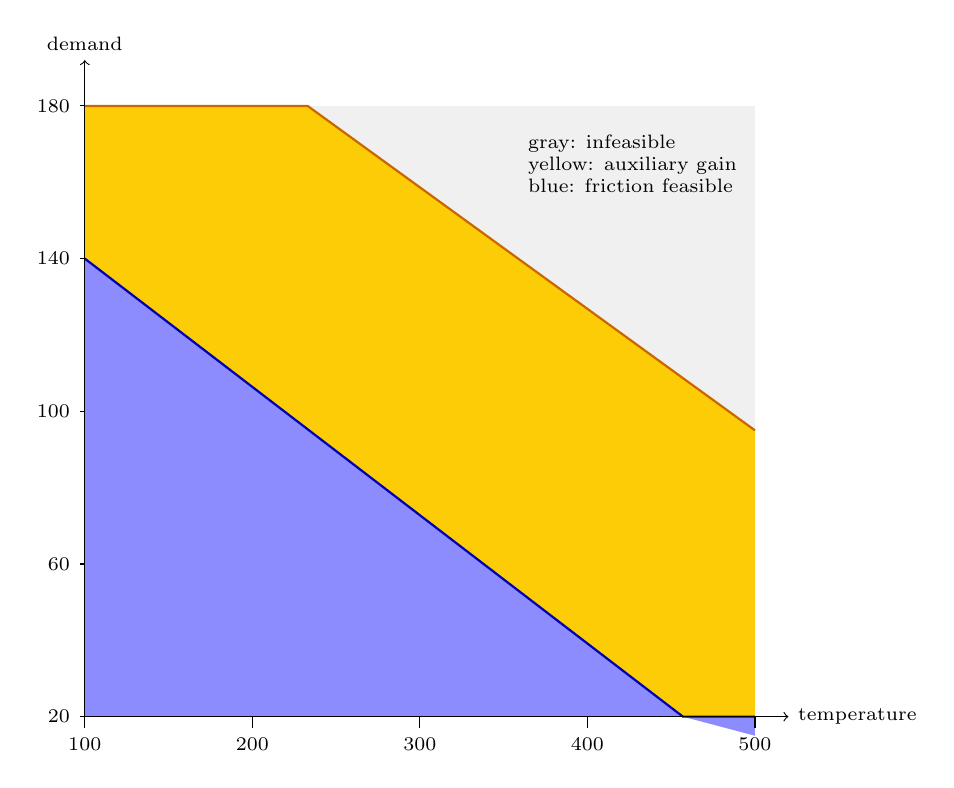
\begin{tikzpicture}[x=0.00175\columnwidth,y=0.0040\columnwidth,font=\scriptsize]
  % Coordinates use x=(T-100) degC and y=(demand-20) kN.
  \fill[gray!12] (0,0) rectangle (400,160);
  \fill[blue!45] (0,0) -- (0,120) -- (357,0) -- cycle;
  \fill[blue!45] (357,0) -- (400,0) -- (400,-5) -- cycle;
  \fill[yellow!65!orange] (0,120) -- (0,160) -- (133,160) -- (400,75) -- (400,0) -- (357,0) -- cycle;
  \draw[thick,blue!70!black] (0,120) -- (357,0) -- (400,0);
  \draw[thick,orange!80!black] (0,160) -- (133,160) -- (400,75);
  \draw[->] (0,0) -- (420,0) node[right]{temperature};
  \draw[->] (0,0) -- (0,172) node[above]{demand};
  \foreach \x/\lab in {0/100,100/200,200/300,300/400,400/500}{\draw (\x,0)--(\x,-3) node[below]{\lab};}
  \foreach \y/\lab in {0/20,40/60,80/100,120/140,160/180}{\draw (0,\y)--(-3,\y) node[left]{\lab};}
  \node[align=left,anchor=north east] at (395,155) {gray: infeasible\\yellow: auxiliary gain\\blue: friction feasible};
\end{tikzpicture}
